\documentclass[tikz,border=4pt]{standalone}
\usepackage{pgfplots}
\usepgfplotslibrary{groupplots,statistics}
\pgfplotsset{compat=1.18}

\definecolor{CDr}{HTML}{CC79A7}
\definecolor{CEq}{HTML}{D55E00}
\definecolor{CFl}{HTML}{0072B2}
\definecolor{CTc}{HTML}{56B4E9}
\definecolor{CVo}{HTML}{E69F00}
\definecolor{CWf}{HTML}{009E73}
\definecolor{COrange}{HTML}{E69F00}
\definecolor{CRed}{HTML}{D55E00}
\definecolor{CBlue}{HTML}{0072B2}

\begin{document}
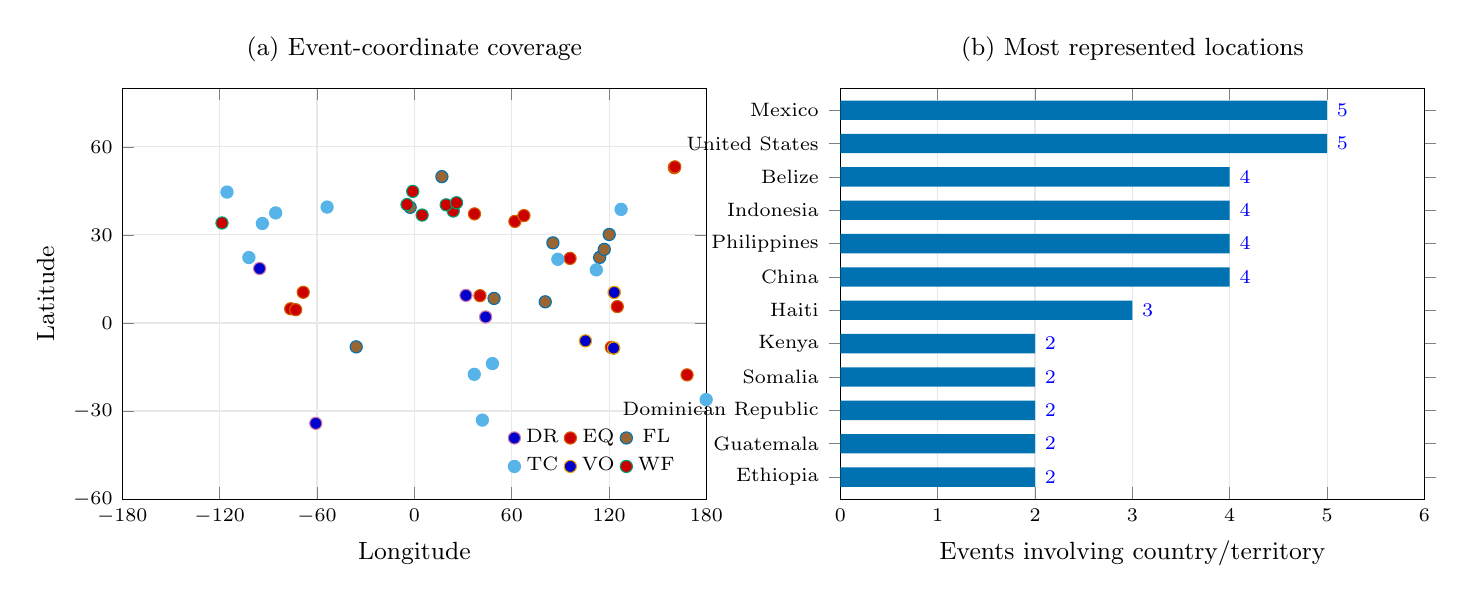
\begin{tikzpicture}
\begin{groupplot}[group style={group size=2 by 1,horizontal sep=1.7cm},
  width=9.0cm,height=6.8cm,tick label style={font=\scriptsize},label style={font=\small},
  title style={font=\small},legend style={font=\scriptsize,draw=none,fill=none}]
\nextgroupplot[xmin=-180,xmax=180,ymin=-60,ymax=80,xtick={-180,-120,-60,0,60,120,180},
  ytick={-60,-30,0,30,60},grid=both,grid style={gray!18},
  xlabel={Longitude},ylabel={Latitude},title={(a) Event-coordinate coverage},
  legend columns=3,legend pos=south east]
\addplot+[only marks,mark=*,mark size=2.2pt,CDr] coordinates {(43.899,2.053) (-95.396,18.563) (-60.785,-34.19) (31.76,9.405)};
\addplot+[only marks,mark=*,mark size=2.2pt,CEq] coordinates {(121.3517,-8.3101) (-68.5139,10.453) (125.0469,5.5918) (168.0338,-17.6859) (-76.2422,4.8436) (160.1413,52.9242) (61.9242,34.6102) (160.5129,53.1928) (95.9216,22.0128) (67.4843,36.5894) (-73.1444,4.5125) (37.032,37.1736) (40.4246,9.2986)};
\addplot+[only marks,mark=*,mark size=2.2pt,CFl] coordinates {(16.9561,49.8591) (80.6401,7.2143) (120.076,30.1534) (85.3649,27.2953) (49.0834,8.3677) (114.1849,22.3506) (-35.8566,-8.1356) (-2.6232,39.4178) (117.0123,25.0767)};
\addplot+[only marks,mark=*,mark size=2.2pt,CTc] coordinates {(-93.7,33.9) (41.87,-33.09) (179.8,-26.1) (88.4,21.7) (-115.5,44.6) (-53.8,39.5) (48.09,-13.83) (36.9,-17.5) (-102.0,22.3) (127.4,38.7) (-85.5,37.5) (112.1,18.1)};
\addplot+[only marks,mark=*,mark size=2.2pt,CVo] coordinates {(123.132,10.412) (122.775,-8.542) (123.132,10.412) (122.775,-8.542) (105.4233,-6.1009)};
\addplot+[only marks,mark=*,mark size=2.2pt,CWf] coordinates {(23.926,38.1512) (19.5897,40.25) (-4.5405,40.3594) (25.9573,40.9741) (-118.5698,34.0804) (-1.0329,44.8463) (4.7743,36.7724)};
\legend{DR,EQ,FL,TC,VO,WF}
\nextgroupplot[xbar,bar width=7pt,symbolic y coords={Ethiopia,Guatemala,Dominican Republic,Somalia,Kenya,Haiti,China,Philippines,Indonesia,Belize,United States,Mexico},ytick=data,
  xmin=0,xmax=6,xtick distance=1,xmajorgrids,grid style={gray!18},
  xlabel={Events involving country/territory},title={(b) Most represented locations},
  nodes near coords,nodes near coords style={font=\scriptsize},
  enlarge y limits=0.06]
\addplot+[xbar,fill=CBlue,draw=none] coordinates {(2,{Ethiopia}) (2,{Guatemala}) (2,{Dominican Republic}) (2,{Somalia}) (2,{Kenya}) (3,{Haiti}) (4,{China}) (4,{Philippines}) (4,{Indonesia}) (4,{Belize}) (5,{United States}) (5,{Mexico})};
\end{groupplot}
\end{tikzpicture}
\end{document}
